% !TEX root = ../../../../temp_manuscript.tex

\chapter[Automated 3D segmentation and diameter measurement of the thoracic aorta on non-contrast enhanced CT][LGG location molecular subgroups]{Automated 3D segmentation and diameter measurement of the thoracic aorta on non-contrast enhanced CT}\label{chap:Aorta_Segmentation}


\begin{ChapterAbstract}
    \textbf{Objectives:} To develop and evaluate a fully automatic method to measure diameters of the ascending and descending aorta on non-ECG-gated, non-contrast computed tomography (\gls{CT}) scans.

    \textbf{Material and methods:}
    The method combines multi-atlas registration to obtain seed points, aorta centerline extraction, and an optimal surface segmentation approach to extract the aorta surface around the centerline. From the extracted 3D aorta segmentation, the diameter of the ascending and descending aorta was calculated at cross-sectional slices perpendicular to the extracted centerline, at the level of the pulmonary artery bifurcation, and at $1-cm$ intervals up to $3 cm$ above and below this level.
Agreement with manual annotations was evaluated by dice similarity coefficient (DSC) for segmentation overlap, mean surface distance (MSD), and intra-class correlation (ICC) of diameters on $100$ CT scans from a lung cancer screening trial. Repeatability of the diameter measurements was evaluated on $617$ baseline-one year follow-up CT scan pairs.

    \textbf{Results:}
   The agreement between manual and automatic segmentations was good with $0.95 /pm 0.01$ DSC and $0.56 /pm 0.08 mm$ MSD. ICC between the diameters derived from manual and from automatic segmentations was $0.97$, with the per-level ICC ranging from $0.87$ to $0.94$. An ICC of $0.98$ for all measurements and per-level ICC ranging from 0.91 to 0.96 were obtained for repeatability.

    \textbf{Conclusions:}
    This fully automatic method can assess diameters in the thoracic aorta reliably even in non-ECG-gated, non-contrast CT scans. This could be a promising tool to assess aorta dilatation in screening and in clinical practice.
    
    \textbf{Key Points:}
    \begin{itemize}
    \item Fully automatic method to assess thoracic aorta diameters.
    \item High agreement between fully automatic method and manual segmentations.
    \item Method is suitable for non-ECG-gated CT and can therefore be used in screening.
	\end{itemize}

    \publishedas{wijnenga2019differencesLGG}
\end{ChapterAbstract}

\section{Introduction}
Aortic aneurysm with the risk of acute dissection is an important cause of mortality in the western world \autocite{roth2015global}. The prevalence of thoracic aortic aneurysms is estimated around $0.3$ percent in the normal population \autocite{itani2002measurement, kalsch2013body}. Most patients with a dilated aorta or aortic aneurysm are asymptomatic. The diagnosis can be made as during screening in the context of a positive family history or by coincidence on imaging examinations performed for other purposes like lung cancer screening \autocite{mets2012computed}. However, acute dissection is often the first presentation, in which case over $50\%$ of all patients die within $30$ days \autocite{melvinsdottir2016incidence}.


Because of this silent process with high risks, screening programs using non-contrast computed tomography (CT) could be considered. In patients with aortic aneurysms, the aortic size has a profound impact on the risk of dissection \autocite{davies2006novel,kim2015risk}. Detecting aortic dilatation at an early stage enables preventive surgery, which might save lives. CT imaging of the thoracic aorta could become available as part of a comprehensive assessment of CT imaging performed for screening purposes including also other organs (lungs,  coronary calcium, vertebral bone density etc.) \autocite{mets2012computed}


By measuring aortic dimensions in such screening cohorts we will also gain more information on normal values of aortic diameters, normal increase in diameters over time, and risk factors for dilatation, and a better insight in prognosis. 

Besides its potential in screening, non-contrast CT is frequently used in diagnosis and follow-up of patients in clinical practice. It plays a central role in the imaging of the thoracic aorta because of the short time required for image acquisition, the ability to obtain a complete 3D view of the entire aorta, and its widespread availability. CT scans can be used for follow-up of patients with dilatation, especially in cases where echocardiography does not adequately visualize the dilatation. The ESC Guidelines and ACCF/AHA guidelines \autocite{american20102010, erbel2014esc} describe standard anatomical landmarks for reporting aortic diameters in CT in clinical practice. 

Performing measurements of the aorta manually is labor intensive and subject to inter-observer variability. To assess aortic dilatation both in screening settings and in clinical practice, automated aorta segmentation and subsequent diameter analysis is therefore desirable. While automatic solutions for aortic measurements in CT angiography (CTA) exist \autocite{gao2017quantification, entezari2013analysis, elattar2014automatic, ecabert2011segmentation, biesdorf2012segmentation}, automatic aorta segmentation in non-contrast CT scans is more challenging due to the lack of contrast between blood pool regions and surrounding soft tissue \autocite{kitasaka2002automated, avila2013segmentation, kurugol2015automated, isgum2009multi, xie2014automated}.


The aim of the current study is to develop and validate an automatic method to robustly assess diameters of the ascending and descending aorta in non-ECG-gated, non-contrast CT without human interaction.


\section{Materials and Methods}

\subsection{Study Population \& Image Acquisition}
The CT scans used in this study are from the Danish Lung Cancer Screening Trial \autocite{pedersen2009danish}. A Multi Detector CT scanner (Mx 8000 IDT 16 row scanner, Philips Medical Systems) was used to acquire CT scans at 120 kV / 40 mAs at maximum inspiration breath hold and without cardiac gating. This protocol leads to an effective dose of around 1 mSv \autocite{wille2016results}. The scans were reconstructed with a sharp kernel (Philips D), in-plane isotropic resolution of $0.78 \times 0.78 mm$, and $1 mm$ slice thickness. Participants were current or former smokers between 50 and 70 years of age. For this study $742$ participants were randomly selected, which were divided into three non-overlapping sets: (see supplementary table S1 for clinical characteristics of the entire data)
\begin{itemize}
\item baseline scans of 25 subjects for parameter optimization of the proposed method;
\item baseline scans of 100 subjects for evaluation of the method’s accuracy (see Table \cref{tab: 1}); 
\item baseline and first year follow up scans of 617 subjects to evaluate the repeatability of the method;
\end{itemize}
    
Therefore, aortic diameter measurements were performed in 1334 CT scans in total. 


\subsection{Manual Annotation}
Manual annotations were made using an in-house annotation tool developed in MeVisLab. 100 CT scans were annotated by a physician (LB) for validation and an additional 25 scans by an experienced observer (ZSG) for method development. The annotation tool was similar to that described previously for carotid artery segmentation in \autocite{hameeteman2011evaluation}. First, the window level/width was adjusted to $200HU/600HU$, for all cases. Then, the aortic centerlines were drawn manually using the axial, coronal and sagittal views, starting from the sinotubular junction of the ascending aorta and ending at the diaphragm level of the descending aorta. Subsequently, the centerlines were checked and modified in reformatted cross-sectional views perpendicular to the drawn centerline. The obtained centerlines were used to generate curved multiplanar reformatted images of the entire aorta, with longitudinal views at six different angles equally spaced every $30\textdegree$ and cross-sectional views every $1 mm$ along the centerline. Longitudinal contours were drawn manually, whereupon cross-sectional contours were computed using spline interpolation through the intersection points of the longitudinal contours with the cross-sectional planes. Finally, after checking the cross-sectional contours in all cross-sections and adjusting them if required, the contours were converted to a 3D binary image using variational interpolation \autocite{heckel2011interactive}. An example of manual annotation is shown in Figure \cref{fig:mannual_Annotation}.

To manually locate the pulmonary artery bifurcation level, an experienced physician (DB) checked the scans in axial view and annotated the pulmonary artery bifurcation level where the left and right pulmonary arteries and the bifurcation from the pulmonary trunk were all visible.

\subsection{Automatic Aorta Segmentation Approach}
To extract a full 3D segmentation of the aorta and a landmark point for the pulmonary artery bifurcation level, we applied a combination of image processing techniques. First, to avoid the segmentation to attract to the heart-lung or bone borders, we applied preprocessing as proposed in our previous work \autocite{sedghi2018aorta}.


Subsequently, a multi-atlas registration method was applied \autocite{kiricsli2010evaluation} to localize the aorta, the pulmonary artery trunk, and the left and right pulmonary arteries. In this method, 25 preprocessed CT scans were non-rigidly registered to the scan in which the
segmentation was required (target image). From these 25 registered images, the ten with the highest similarity to the target image were selected. The corresponding manual annotations of these ten scans were then deformed and combined using a per voxel majority voting procedure to obtain a coarse initial segmentation of the aorta and pulmonary arteries. The initial segmentation of the pulmonary arteries was then skeletonized, and the slice where main pulmonary artery bifurcates into the left and right pulmonary arteries was extracted as the pulmonary
artery bifurcation level. This level is used as the landmark level.


To start tracing the centerline of the aorta, aortic seed points were extracted as the center of mass of the coarse initial aorta segmentation at the axial slice 3 cm beneath the landmark level for the ascending aorta and 6 cm beneath the landmark level for the descending aorta. The aortic centerline was then extracted between these seed points by a minimum cost path tracking algorithm similar to \autocite{sedghi2018aorta}. In this algorithm, the cost function was based on the maximum output of a multi-radius medialness filter in coronal and axial views multiplied with a lumen intensity similarity metric. The centerlines were refined by re-computing the minimum cost path after curved multiplanar reformatting perpendicular to the previous centerline \autocite{tang2012semiautomatic}. Failure in the centerline extraction was automatically detected by using the landmark level and the initial pulmonary artery segmentation. Centerlines that did not reach the landmark level or were inside the pulmonary artery segmentation were considered failed extractions and were excluded.


To obtain a first estimate of the aorta, the extracted centerline was dilated using a spherical structuring element with its radius defined by the estimated radius of the aorta obtained from the medialness filter. Subsequently, an optimal surface graph cut segmentation method\footnote{Available at https://bitbucket.org/opfront/opfront} \autocite{petersen2014optimal}, initialized by the dilated centerline, was used to accurately extract the surface of the aorta. The parameters for atlas registration, centerline extraction, and graph cut segmentation were tuned to maximize the similarity with manual annotations on 25 CT scans.

\subsection{Aortic Diameter Measurement}
Aortic diameters were assessed at multiple, fixed levels relative to the pulmonary artery bifurcation level. Based on the extracted pulmonary bifurcation level, thirteen cross-sectional slices were defined perpendicular to the extracted aortic centerline, located at 1-cm intervals around the bifurcation level from 2 cm below this level to 3 cm above for the ascending aorta and from 3 cm above to 3 cm below this level for the descending aorta. For the ascending aorta, the cross-sectional slice at 3 cm below the pulmonary artery bifurcation level was sometimes in the aortic root below the sinotubular junction which the aorta boundaries at the sinus of Valsalva are very unclear due to the lack of gating and contrast. Therefore, no measurements were performed at this level. Figure \cref{fig:3D_Diameter} shows an example of 3D segmentation with the corresponding centerline and four of the measured cross-sections.


The cross-sectional average aortic diameter at each of the 13 cross-sectional slices was computed from manual and automatic segmentations. For the manual segmentations, diameter measurements were performed perpendicular to the manual centerlines and at levels relative to the manually indicated pulmonary artery bifurcation level. For the automatic segmentations, the automatically extracted centerlines and pulmonary artery bifurcation level were used instead.


\subsection{Validation and Statistical analysis}
The method was validated on 100 CT scans with manual annotations. The segmentation accuracy was assessed by dice
similarity coefficient (DSC) and mean surface distance (MSD). DSC \autocite{dice1945measures} measures the degree of spatial overlap of the automatic segmentation with the manual segmentation,and it ranges between 0 and 1, where higher values indicate higher similarity. MSD shows the symmetric mean surface distance in millimeters between the manual and automatic segmentation surfaces, where lower value is better. The agreement between the manual and automatic segmentations was assessed from $3 cm$ beneath the landmark level at the ascending aorta to 6 cm beneath this level at the descending aorta. DSC, MSD, aortic diameters, and the error in the diameter
were expressed as mean $\pm$ standard deviation (range).


The error in the extracted landmark level was assessed by the distance between the manually extracted pulmonary artery bifurcation level and the automatically extracted level in millimeters. The aortic centerlines were automatically checked for failed extractions.

The agreement between the manual and automatic diameter measurements was assessed by 
\begin{enumerate}
\item intra-class correlation (ICC) based on a single-rating, absolute-agreement, two-way mixed-effects model \autocite{koo2016guideline}; 
\item R$^2$ Pearson’s correlation;
\item Bland-Altman analysis;
\end{enumerate}

Repeatability of the method was assessed by comparing the automatically extracted diameters of two scans of 617 subjects with time period of 1 year in between. Within 1 year, changes in aortic diameters are expected to be small, with 0.1–0.2-mm growth per year in a healthy population \autocite{kalsch2013body, davies2006novel}. All statistical analyses were done in MATLAB.



\section{Results}
Figure \cref{fig:segmentation_Sample} shows examples of segmentation results. Out of all 1334 CT scans only in two cases, the seed points at the descending aorta were extracted incorrectly. Centerline extraction further failed in seven cases, all of which were easily detected automatically. Average DSC for the entire aorta was $0.95 \pm 0.01$ (0.92–0.96) and MSD was $0.56 \pm 0.08$ (0.43–0.93) mm. The mean absolute distance between the manual and automatic landmark level of the pulmonary artery bifurcation was $2.55 \pm 1.94 mm$, with almost no bias (mean signed distance $0.45 \pm 3.18 mm$).


Box plots for the average manual and automatic diameters for each measuring level are shown in Figure \cref{fig: Boxplot_Diameter}. Diameters measured at the different levels, for men and women separately, are shown in Table \cref{tab: table 2}. High agreement between manually and automatically measured diameters was obtained, with an overall ICC and R$^2$ Pearson’s correlation of 0.97. The level-wise correlations together with the correlations separated per gender are shown in Table \cref{tab: TAble 3 } (see supplementary Figure \cref{fig:Supplimentary_S1 } for scatter plots of each measuring level).

An average absolute diameter error of $1.09 \pm 0.6 mm$ between manual and automatic diameters was obtained over all measuring levels, which 
showed a slight underestimation of the automated measurements compared to manual measurements (mean signed error -  $0.97 \pm 0.8 mm$). As shown in box plots of the level-wise diameter errors in Figure \cref{fig:Boxplot_Difference}, larger errors (more than 3 mm) were extracted in 8 out of 100 scans. In four cases, a large error occurred due to motion artifacts at the ascending aorta (beneath the landmark level), and in three cases, it occurred at the aortic arch due to branching arteries. In one case, the error was along the entire aorta due to a 6-mm difference between the automatic and manual landmark levels. Bland-Altman plots of manual and automated diameter measurements are given in Figure \cref{fig:Bland_Altman}.


From the 617 subjects used to assess repeatability, 7 subjects had failed centerline or seed point extraction. From the remaining 610 subjects, ICC between the automatic diameters of the scan and rescan of each subject is shown in Table \cref{tab: table 4}. From these 610 subjects, 72 subjects ($12\%$) had an absolute diameter difference larger than $3 mm$ between the two time points at any of the measuring levels. In 35 out of 72 cases ($48.6\%$), the segmentations appeared visually correct in both time points. In 17 cases of these 35 cases, a 2- or 3-mm difference between the extracted landmark level in one of the time points resulted in big diameter differences at 2 cm below the landmark level at the ascending aorta (in average $3.7 \pm 0.5 mm$). This is due to the aortic anatomy at the sinotubular junction where the aorta below this level is on average 3 mm larger than above \autocite{vriz2013aortic}. In 5 out of 35 cases, there was more than 6-mm difference between the extracted landmark levels from the two time points, leading to a diameter measure ment at very different levels along the entire aorta being compared (in average $3.4 \pm 0.5 mm$). The remaining 13 out of 35 cases appeared to have a slightly larger diameter at one of the time points (in average $3.7 \pm 0.7 mm$), possibly due to the aortic size changes during the cardiac cycle. In 37 out of 72 cases ($51.4\%$), the average diameter difference ($3.6 \pm 0.6 mm$) was due to segmentation error which mainly occurred at the aortic arch which was due to branching arteries, or was at the ascending aorta below the pulmonary artery bifurcation level which was due to heart motion artifacts caused by the non-ECG-gated data.


\section{Discussion}

We presented a fully automatic method to segment the thoracic aorta and measure aortic diameters. In our evaluation on 100 non-ECG-gated, non-contrast CT scans, the 3D segmentation algorithm performed well with an average segmentation overlap of $0.95 \pm 0.01$ and a mean surface distance between manual and automatic segmentations of less than 1 voxel (0.56 mm).


The agreement with diameters obtained from manual segmentations was high, with an overall ICC of 0.97 and an average per-level ICC of $0.91 \pm 0.03$, which is similar to the agreement reported between observers in \autocite{terzikhan2017pulmonary} (ICC = 0.94). The manual diameters were on average approximately 1 mm larger than automatic diameters. This bias is similar to interobserver bias reported in \autocite{quint2013proximal} for mid-ascending aorta diameter measurement on CTA. Scan-rescan repeatability was high, with an overall ICC of 0.98 and an average per-level ICC of $0.94 \pm 0.01$.


The mean ascending aorta diameters measured at the pulmonary artery bifurcation level were $36.7 \pm 3.5 mm$ for males and $33.9 \pm 3.3 mm$ for females. These values are similar to those reported by Kalsch et al \autocite{kalsch2013body} ($37.1 \pm 4 mm$ for males and $34.5 \pm 4 mm$ for females), while they were slightly greater than those reported by Wolak et al \autocite{wolak2008aortic} ($33.5 \pm 4 mm$ for males and $31.4 \pm 3 mm$ for females). These differences may be due to differences in the study populations, CT scan protocol, and measurement approach.


A significant diameter increase of on average $0.11 \pm 1.0 mm$ was measured in repeated scans after 1 year. This agrees well with reported natural yearly aortic diameter growth of 0.1 – 0.2 mm per year in the healthy population \autocite{kalsch2013body, davies2002yearly}. In $12\%$ of repeat scan pairs (72 subjects), diameter changes larger than 3 mm were observed. In the majority of these cases (44 subjects), large diameter differences occur at the ascending aorta beneath the landmark level which is due to the anatomy and the difficulty of measuring these regions. Due to motion artifacts in the non-ECG-gated scans, segmentation of the proximal part of the aorta including the aortic root is difficult even for experienced radiologists. However, although isolated aortic root aneurysms are seen in patients with Marfan syndrome \autocite{authors20142014}, it is less common than aneurysms of the ascending aorta more distal to the aortic root. Therefore, the aortic root segmentation is less important in our application than the ascending aorta. In the remaining 28 cases, the large diameter difference was either in the aortic arch (15) or in the descending aorta (8) or at multiple locations due to error in the extraction of the pulmonary artery bifurcation level (5). Diameters measured at the aortic arch were visually correct; however, slightly larger diameters were measured at the location of branching arteries. In descending aorta, the large diameter differences were mainly due to segmentation error.


In contrast with our study, in literature, most methods for automatic aorta segmentation were evaluated on CTA in which the aortic lumen is much more clearly visible \autocite{gao2017quantification, entezari2013analysis, elattar2014automatic, ecabert2011segmentation, biesdorf2012segmentation}. Few methods were proposed to segment the aorta in non-contrast CT \autocite{kitasaka2002automated, avila2013segmentation, kurugol2015automated, isgum2009multi, xie2014automated}. Compared to these previous works, shown in Table \cref{ tab: table 5}, our proposed method is evaluated on a larger dataset and shows better performance.


We proposed to measure aortic dimensions at fixed intervals with respect to a single anatomical landmark level, the pulmonary artery bifurcation. In clinical practice, multiple anatomical landmarks including locations in the aortic arch are used instead for reporting aortic diameters in CTA \autocite{american20102010, authors20142014, hager2002diameters}. However, consistently extracting these landmarks especially in non-ECG-gated CT is difficult. Moreover, the aorta diameter is poorly defined at the locations of the brachiocephalic artery, left-common carotid artery, and left-subclavian artery. Consistent measurements in the arch require landmark points in between branches that are not affected by this issue; however, detecting such points automatically and robustly in non-contrast CT scans is difficult. Furthermore, aortic dilatation is less common in the arch than in the ascending and descending aorta. Therefore, in this paper, we focus on the ascending and descending aortas which clinically are of more interest. In non-contrast CT, diameters have been mainly measured at the pulmonary artery bifurcation level \autocite{itani2002measurement, kalsch2013body, wolak2008aortic, mao2008normal, lin2008assessment}. The measuring levels used in our study approximately cover the same area used in CTA \autocite{american20102010, authors20142014, hager2002diameters} but are easier to extract reliably in non-contrast and non-ECG-gated CT.


A limitation of our study is that the method was validated only on a relatively healthy screening population. Further investigation would be required to evaluate the performance on abnormal aortic shapes or large aneurysms. However, in all cases with aortic dilatation as indicated in the original radiology reports, the obtained segmentation was correct. In our data, calcification in the aorta was assessed by the Agatston
score \autocite{rasmussen2013relationship}. Visual inspection of the scans with Agatston score higher than 1500 for the entire aorta (58 out of 742 subjects) showed that the proposed method segmented the calcifications correctly inside the vessel wall in all cases.


The proposed automatic method is a promising technique to accurately and reproducibly assess subtle signs of aorta dilatation in non-ECG-gated, non-contrast CT scans without any human interaction and could be used for efficient screening for aortic dilatation as well as for monitoring of aortic change in clinical practice as part of a comprehensive CT analysis including lung screening.

%%%%%%%
%
%\begin{table}[htbp]
%\scriptsize
%\centering
%\begin{tabular}{L{2.65cm} C{.65cm} C{.65cm} C{.65cm} C{.65cm} C{.65cm} C{.65cm} C{.65cm} C{.65cm}}
%    \toprule
%     & \multicolumn{2}{c}{\bfseries{\thead{Total cohort \\ (N = 224)}}} & \multicolumn{2}{c}{\bfseries{\thead{Oligodendroglioma\\ (N = 92)}}} & \multicolumn{2}{c}{\bfseries{\thead{Astrocytoma\\ \acrshort{IDH} mutated\\ (N = 110)}}} & \multicolumn{2}{c}{\bfseries{\thead{Astrocytoma\\ \acrshort{IDH} wild-type\\ (N = 22)}}}\\
%    \cmidrule{2-9}
%    \bfseries{Characteristics} & N & \% & N & \% & N & \% & N & \%\\
%    \midrule
%    \bfseries{Sex}\\
%    \hspace{1em} Male & 133 & 59.4 & 47 & 51.1 & 70 & 60.9 & 16 & 72.7\\
%    \hspace{1em} Female & 91 & 40.6 & 45 & 48.9 & 40 & 36.4 & 6 & 27.3\\
%
%    \bfseries{Age (years)}\\
%    \hspace{1em} Median & \multicolumn{2}{c}{42} & \multicolumn{2}{c}{45} & \multicolumn{2}{c}{37} & \multicolumn{2}{c}{59}\\
%    \hspace{1em} \acrshort{IQR} & \multicolumn{2}{c}{33-51} & \multicolumn{2}{c}{37-52} & \multicolumn{2}{c}{29-45} & \multicolumn{2}{c}{52-63}\\
%    \hspace{1em} $<40$ & 99 & 44.2 & 32 & 34.8 & 67 & 60.9 & 0 & 0 \\
%    \hspace{1em} 40-60 & 101 & 45.1 & 49 & 53.3 & 41 & 37.3 & 11 & 50\\
%    \hspace{1em} $>60$ & 24 & 10.7 & 11 & 12 & 2 & 1.8 & 11 & 50\\
%
%    \hangindent=.5em\bfseries{Presenting symptom}\\
%    \hspace{1em} Epilepsy & 167 & 74.6 & 76 & 82.6 & 81 & 73.6 & 10 & 45.5\\
%    \hspace{1em} Incidental & 23 & 10.3 & 8 & 8.7 & 14 & 12.7 & 1 & 4.5\\
%    \hspace{1em} Headache & 8 & 3.6 & 1 & 1.1 & 6 & 5.5 & 1 & 4.5\\
%    \hspace{1.3em}\hangindent=2em Miscellaneous neurologic complaints & 26 & 11.6 & 7 & 7.6 & 9 & 8.2 & 10 & 45.5\\
%
%    \hangindent=.5em\bfseries{Type of 1st surgery}\\
%    \hspace{1em} Awake craniotomy & 103 & 46 & 49 & 53.3 & 53 & 48.2 & 1 & 4.5\\
%    \hspace{1em} Normal resection & 74 & 33 & 23 & 25 & 48 & 43.6 & 3 & 13.6\\
%    \hspace{1em} Open biopsy & 15 & 6.7 & 7 & 7.6 & 2 & 1.8 & 6 & 27.3\\
%    \hspace{1.3em}\hangindent=2em Stereotactic biopsy & 32 & 14.3 & 13 & 14.1 & 7 & 6.5 & 12 & 54.5\\
%
%    \bfseries{Preoperative \acrshort{KPS}}\\
%    \hspace{1em} Median & \multicolumn{2}{c}{100} & \multicolumn{2}{c}{100} & \multicolumn{2}{c}{100} & \multicolumn{2}{c}{90}\\
%    \hspace{1em} \acrshort{IQR} & \multicolumn{2}{c}{90-100} & \multicolumn{2}{c}{100-100} & \multicolumn{2}{c}{90-100} & \multicolumn{2}{c}{82-90}\\
%    \hspace{1em} 100 & 145 & 64.7 & 70 & 76.1 & 70 & 63.6 & 5 &22.7\\
%    \hspace{1em} 90 & 61 & 27.2 & 17 & 18.5 & 33 & 30 & 11 & 50\\
%    \hspace{1em} $\leq$ 80& 18 & 8 & 5 & 5.4 & 7 & 6.4 & 6 & 27.3\\
%
%    \bfseries{Eloquent area} & 90 & 40.2 & 35 & 38 & 39 & 35.5 & 16 & 72.7\\
%
%    \bfseries{Side of lesion}\\
%    \hspace{1em} Right & 95 & 42.4 & 37 & 40.2 & 51 & 46.4 & 7 & 31.8\\
%    \hspace{1em} Left & 117 & 52.2 & 50 & 54.3 & 57 & 51.8 & 10 & 45.5\\
%    \hspace{1em} Bilateral & 12 & 5.4 & 5 & 5.4 & 2& 1.8 & 5 & 22.7\\
%
%    \hangindent=.5em \bfseries{Preoperative tumor volume (cm$^3$)}\\
%    \hspace{1em} $<$ 25.0 & 64 & 28.6 & 26 & 28.3 & 31 & 28.2 & 7 & 31.8\\
%    \hspace{1em} 25.1-50.0 & 54 & 24.1 & 24 & 26.1 & 24 & 21.8 & 6 & 27.3\\
%    \hspace{1em} 50.1-100.0 & 65 &29 & 23 & 25 & 38 & 34.5 & 4 & 18.2\\
%    \hspace{1em} 100.1-250.0 & 38 & 17 & 17 & 18.5 & 16 & 14.5 & 5 & 22.7\\
%    \hspace{1em} 250.1-351.0 & 3 & 1.3 & 2 & 2.2 & 1 & 0.9 & 0 & 0\\
%    \hspace{1em} Median & \multicolumn{2}{c}{47.3} & \multicolumn{2}{c}{45.9} & \multicolumn{2}{c}{50.95} & \multicolumn{2}{c}{38.2}\\
%    \hspace{1em} Range & \multicolumn{2}{c}{3.01-350.5} & \multicolumn{2}{c}{4.29-350.5}& \multicolumn{2}{c}{3.01-302.8} & \multicolumn{2}{c}{9.05-213.1}\\
%
%    \hangindent=.5em \bfseries{Postoperative tumor volume (cm$^3$)}\\
%    \hspace{1em} 0.0 & 33 &14.7 & 15 & 16.3 & 17 &15.5&1 & 4.5\\
%    \hspace{1em} 0.1-5.0 & 5& 24.1& 27 & 29.3 & 26& 23.6 & 1 & 4.5\\
%    \hspace{1em} 5.1-10.0 & 21& 9.4 & 6& 6.5 & 13 & 11.8 & 2 & 9.1\\
%    \hspace{1em} 10.1-50.0 & 66 & 29.5 & 19 & 20.7 & 38 & 34.5 & 9 & 40.9\\
%    \hspace{1em} 50.1-265.0 & 50 &22.3 & 25 & 27.2 & 16 & 14.5 & 9 & 40.9\\
%    \hspace{1em} Median & \multicolumn{2}{c}{11} &\multicolumn{2}{c}{7.13} & \multicolumn{2}{c}{9.26} & \multicolumn{2}{c}{31.5}\\
%    \hspace{1em} Range & \multicolumn{2}{c}{0-263.6} & \multicolumn{2}{c}{0-263.6} & \multicolumn{2}{c}{0-232.7} & \multicolumn{2}{c}{0-213.1}\\
%
%    \bfseries{Follow-up (years)}\\
%    \hspace{1em} Median & \multicolumn{2}{c}{5.8} & \multicolumn{2}{c}{7.3} & \multicolumn{2}{c}{5.7} & \multicolumn{2}{c}{2.2}\\
%    \hspace{1em} Range & \multicolumn{2}{c}{0.3-20.4} & \multicolumn{2}{c}{0.8-20.4} & \multicolumn{2}{c}{0.3-15}& \multicolumn{2}{c}{0.3-4.7}\\
%    \bottomrule
%\end{tabular}
%\caption{Population demographics and tumor characteristics. Abbreviations: \acrcaption{KPS}, \acrcaption{IQR}}
%\label{tab:LGG_location_characteristics}
%\end{table}



\begin{figure}
\centering
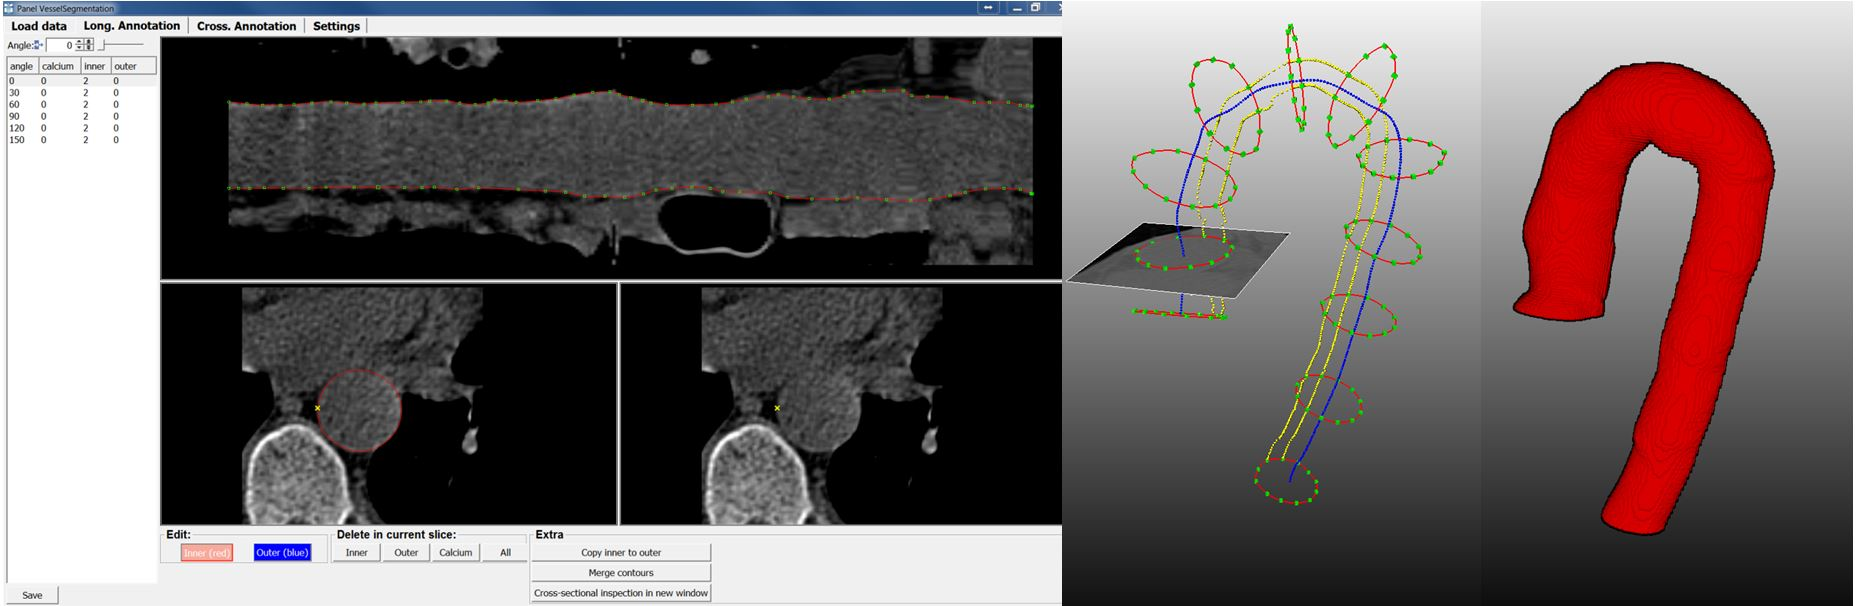
\includegraphics[width=\textwidth]{Figures/Figure1.JPG}
\caption{Screenshot of the manual annotation tool (left). Middle image shows two manually drawn longitudinal contours (yellow) and a few cross-sectional contours (red), which are perpendicular to the manual centerline (blue). A cross-sectional slice at the ascending aorta and the corresponding contour is shown as well. The corresponding 3D surface of the aorta is shown on the right image.}
\label{fig:mannual_Annotation}
\end{figure}


\begin{figure}
\centering
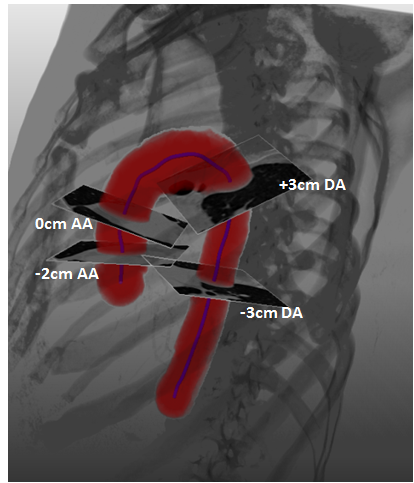
\includegraphics[width=\textwidth]{Figures/Figure2.PNG}
\caption{3D automatic segmentation of the aorta and the corresponding automatic centerline showing cross-sections at the ascending aorta at the pulmonary artery bifurcation level (0 cm AA) and at 2 cm below this level (-2 cm AA) and at the descending aorta at 3 cm above (+3 cm DA) and below (-3 cm DA) the pulmonary artery bifurcation level.}
\label{fig:3D_Diameter}
\end{figure}


\begin{figure}
\centering
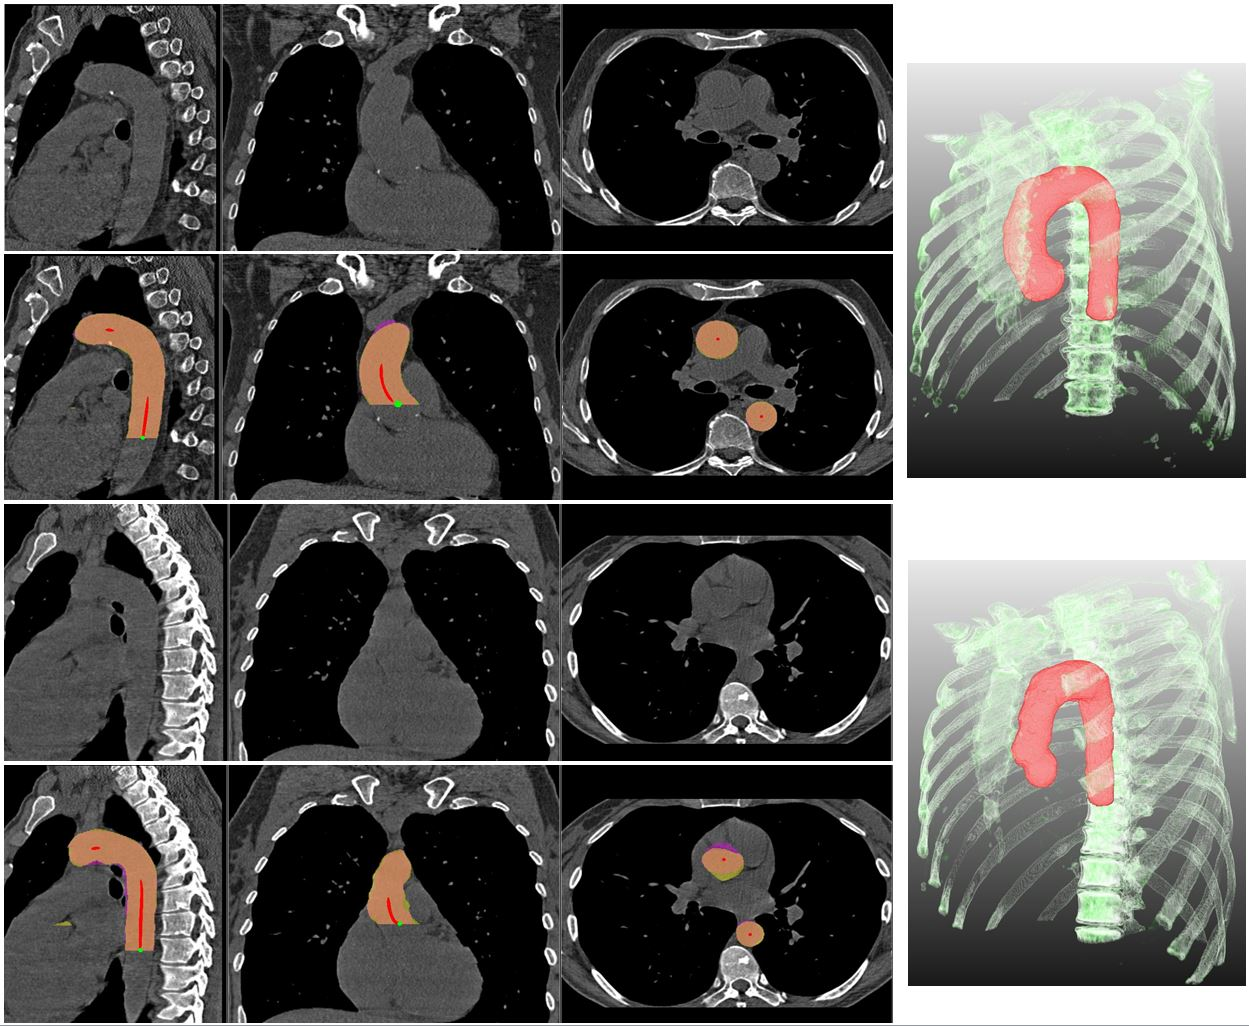
\includegraphics[width=\textwidth]{Figures/Figure3.JPG}
\caption{Two samples with the best (top two rows) and the worst (bottom two rows) automatic segmentation results. The columns from left show the sagittal, coronal, and axial views, respectively. The right column shows the 3D visualization of the automatic segmentation in red. First and third rows are the original CT scans, while the second and fourth rows show the CT scan with the overlap of the corresponding manual and automatic segmentations with DSC = 0.96 and MSD = 0.60 mm for the first sample and DSC = 0.92 and MSD = 1.44 mm for the second sample. Orange shows the regions where the manual and automatic segmentations overlap. Magenta is the region included in the automatic segmentation, but not in the manual segmentation, and yellow is the region that is inside the manual segmentation, but not in the automatic segmentation. Centerline points are indicated in red and seed points in green.}
\label{fig:segmentation_Sample}
\end{figure}

\begin{figure}
\centering
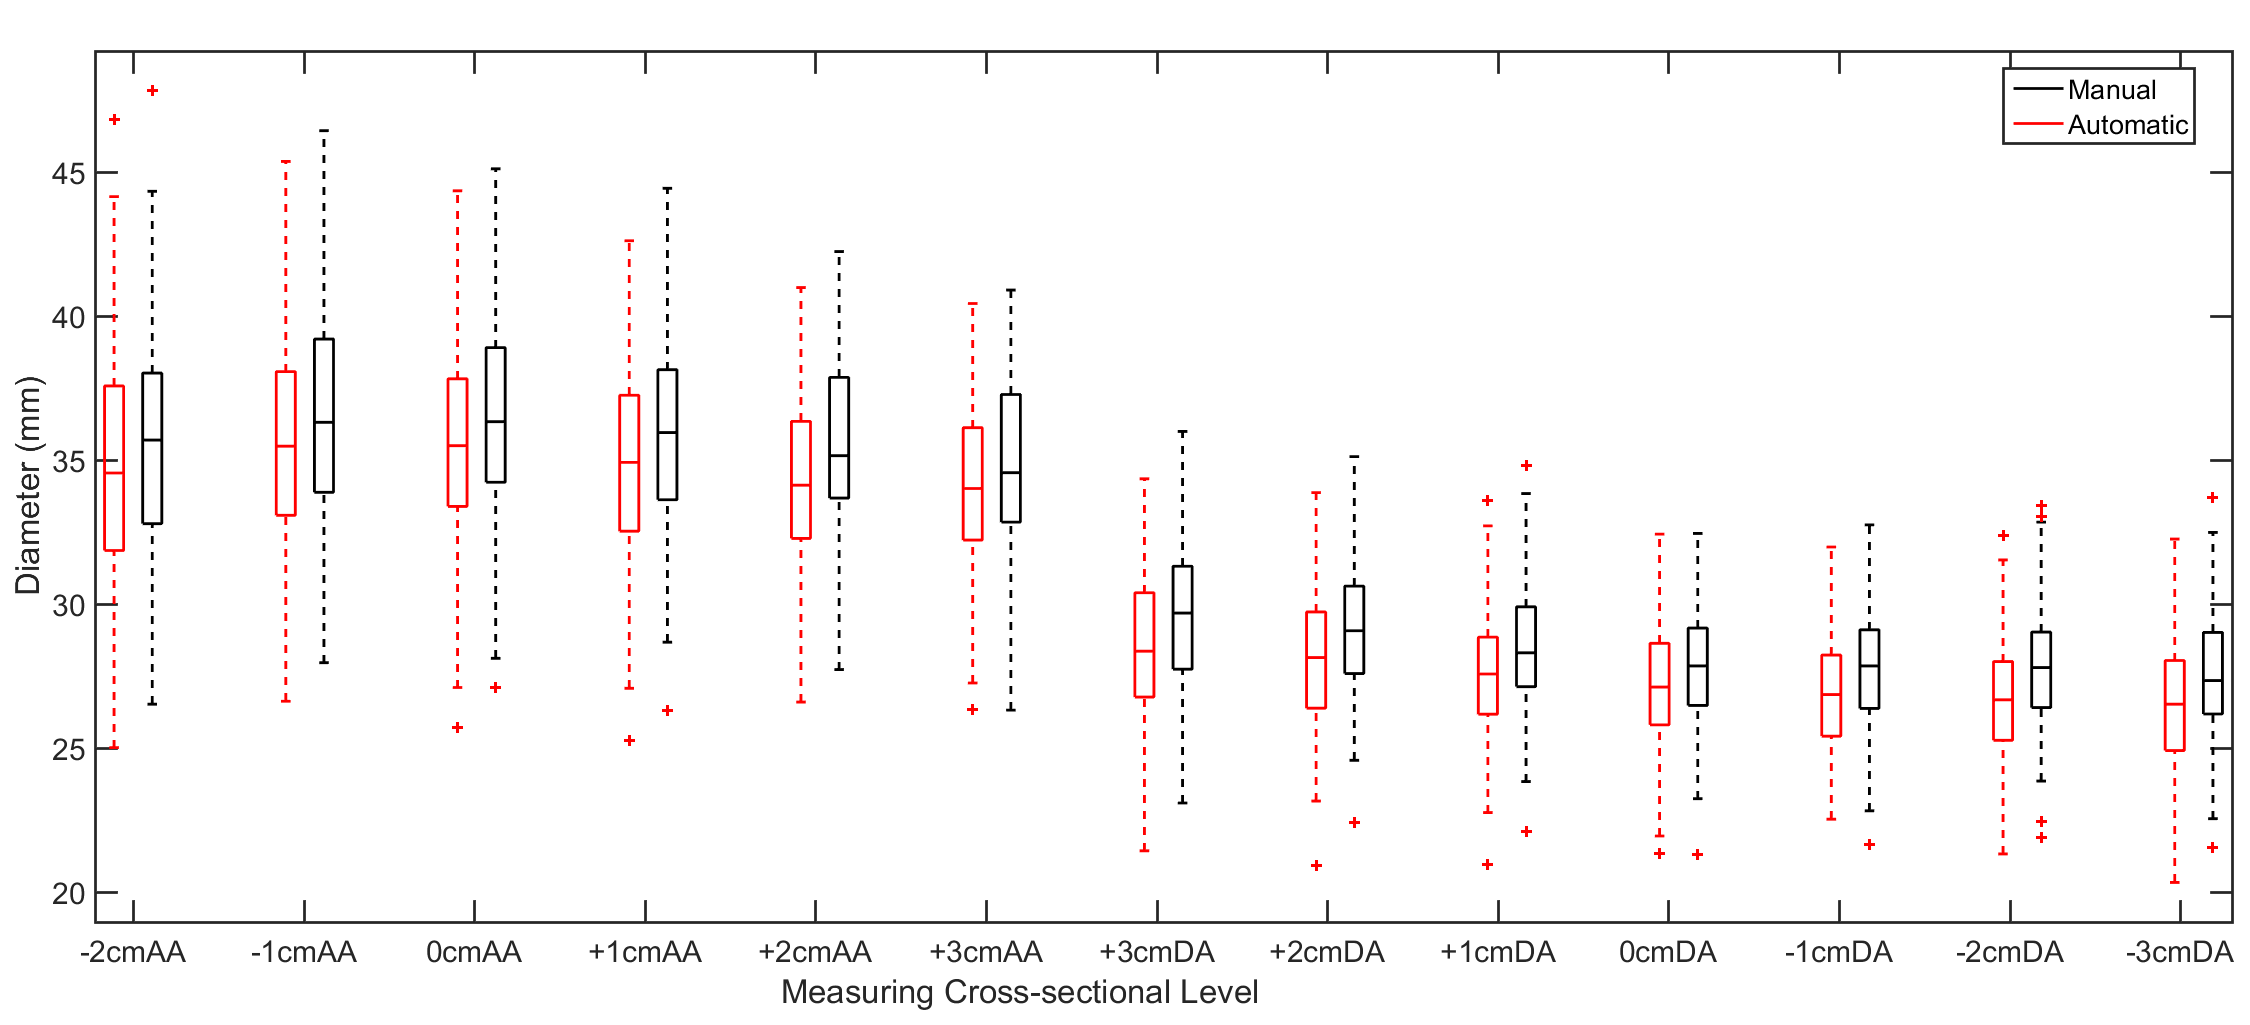
\includegraphics[width=\textwidth]{Figures/Figure4.jpg}
\caption{Average manual (black) and automatic (red) diameter per measuring level. From left to right, diameters measured at the different levels along the aorta from 2 cm below the pulmonary artery bifurcation level (0 cm) at the ascending aorta (AA) to 3 cm below the pulmonary artery
bifurcation level at the descending aorta (DA).}
\label{fig:Boxplot_Diameter}
\end{figure}


\begin{figure}
\centering
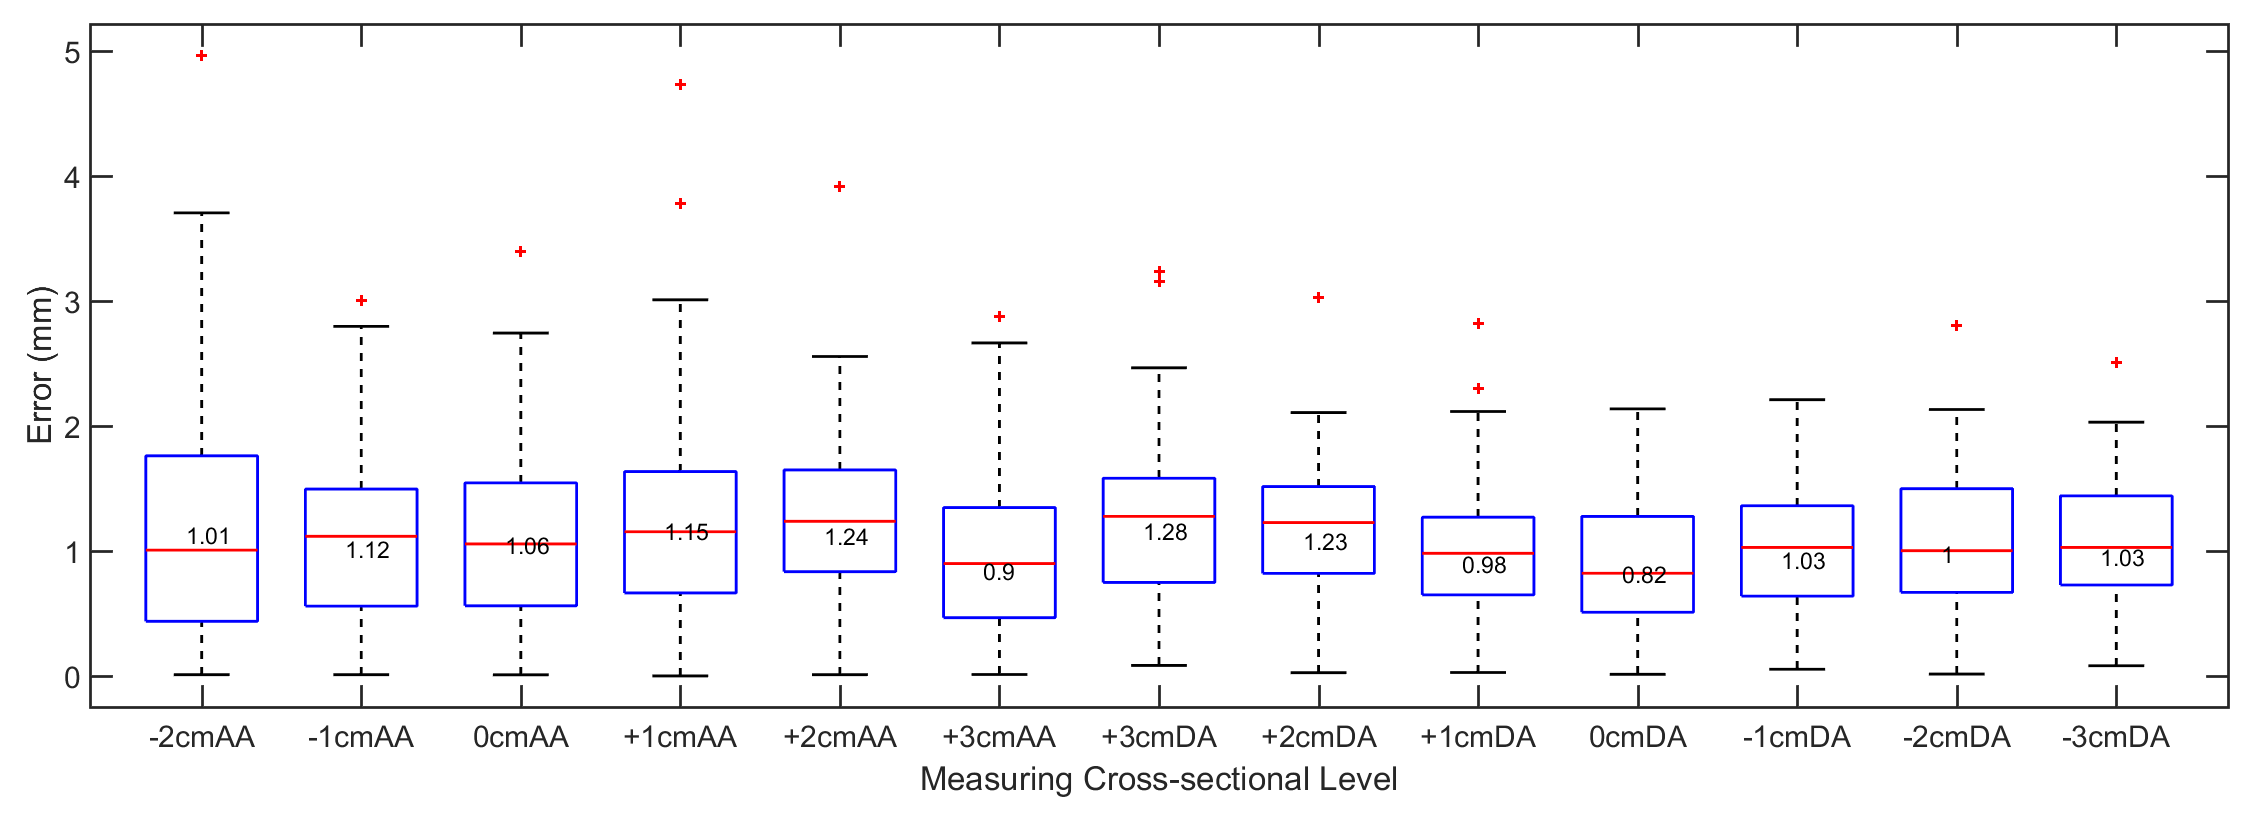
\includegraphics[width=\textwidth]{Figures/Figure5.jpg}
\caption{Absolute difference between the aortic diameters obtained from automated and manual 3D segmentations. From left to right, diameters measured at the different levels along the aorta from 2 cm below the pulmonary artery bifurcation level (0 cm) at the ascending aorta (AA) o 3 cm below the pulmonary artery bifurcation level at the descending aorta (DA). The box plot shows the median (red line), interquartile range (boxes), the $99.3\%$ coverage of the data (whiskers), and the outliers (+ symbol).}
\label{fig:Boxplot_Difference}
\end{figure}


\begin{figure}
\centering
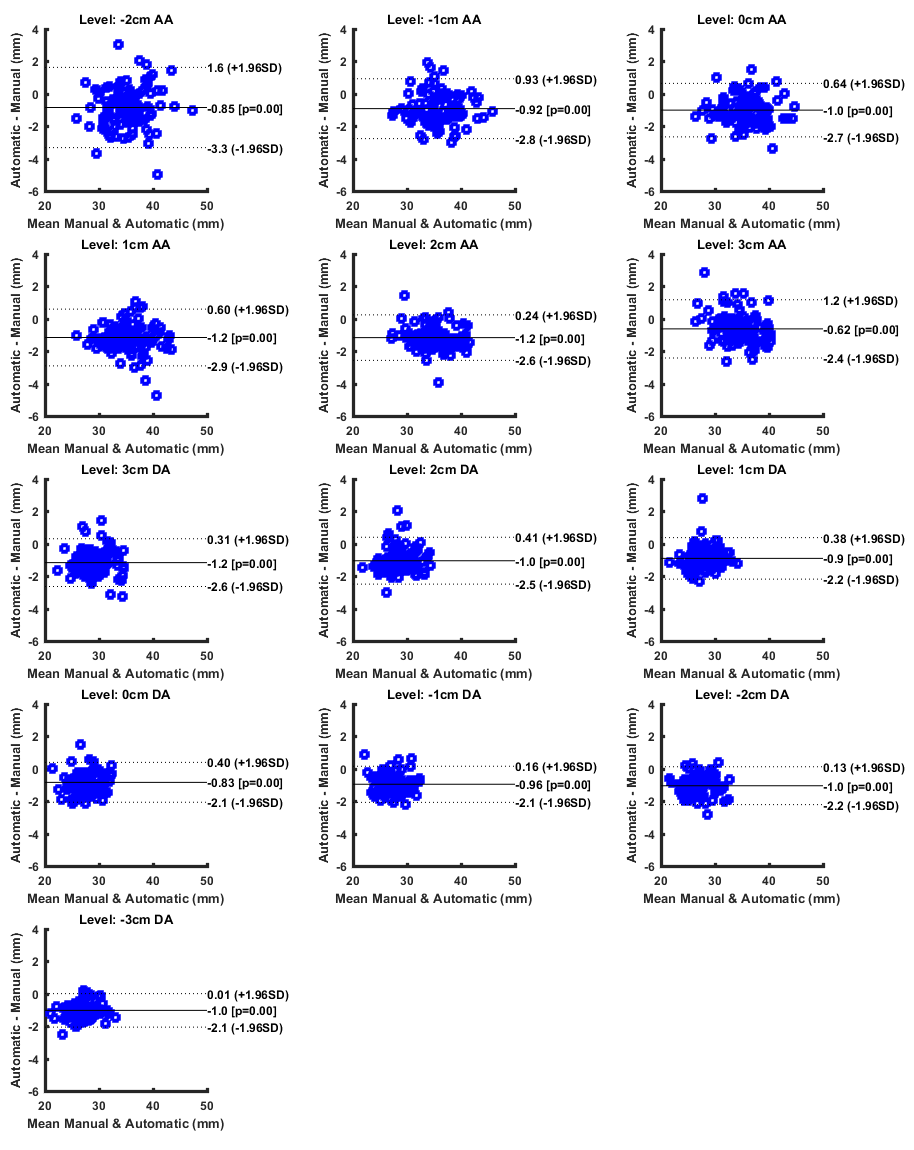
\includegraphics[width=\textwidth]{Figures/Figure6.jpg}
\caption{Bland-Altman plots for each measuring level from 2 cm below the pulmonary artery bifurcation in the ascending aorta (AA) until 3 cm below this level in the descending aorta (DA). The measuring level, limits of agreement, and the mean difference are displayed on the plots.}
\label{fig:Bland_Altman}
\end{figure}


\newpage
\begin{subappendices}
    \section{Supplemental Figures}

    \begin{figure}[htb]
        \centering
        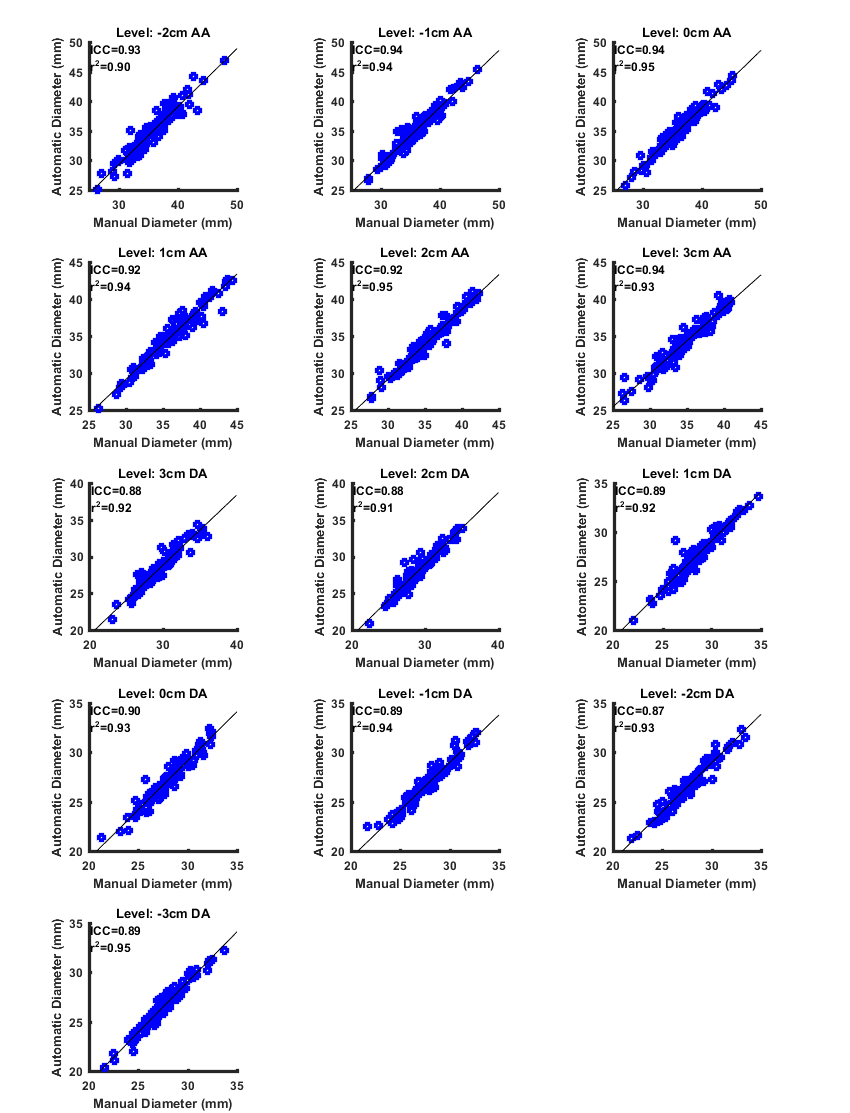
\includegraphics[width=\textwidth]{Figures/Supplemental figure 1.jpg}
        \caption{Scatter plots for each measuring level from 2 cm below the pulmonary artery bifurcation in the ascending aorta (AA) until 3 cm below this level in the descending aorta (DA). The measuring level, ICC, and the R2 Pearson correlation.}\label{fig:Supplimentary_S1}
    \end{figure}

\end{subappendices}
